%%% Beamber preamble - June 2015 %%%
% FR version

\documentclass[t]{beamer} % Top-aligned slides

%% Font & language
\usepackage[utf8x]{inputenc}
\usepackage[frenchb]{babel}
\usepackage[T1]{fontenc}
\usepackage{lmodern}
%\PrerenderUnicode{éàèê}

%% Packages: math, symbols
%\usepackage{gensymb} % for \celsius command
\usepackage{amsmath}
\usepackage{amssymb}
\usepackage{textcomp} % Symbole Euro €
\newcommand{\euro}{\texteuro}
%\usepackage{fixltx2e} % for \textsubscript command


%% Beamer customization:
\usetheme{Frankfurt}
\usecolortheme{beaver} % red & gray colors
% enlever l'ombre sous le titre: (http://tex.stackexchange.com/a/3182/51609)
\setbeamertemplate{title page}[default][colsep=-4bp,rounded=true]
% enlever l'ombre sous toutes les boîtes
\setbeamertemplate{blocks}[rounded][shadow=false]

%\setbeamertemplate{mini frames}{} % remove subsection circles

% Puces :
\setbeamertemplate{itemize items}{$\circ$}
\setbeamertemplate{enumerate items}[default]
\setbeamertemplate{section in toc}[sections numbered]
\setbeamertemplate{subsection in toc}[square]

% Frame number
\setbeamertemplate{footline}[frame number]
\setbeamertemplate{sidebar right}{} % (removes the navigation bar)




%% Custom commands

% Mathematical Expectation E[X] and Covariance
\newcommand\E[1]{\mathbb{E}[#1]}
\newcommand\avg[1]{\langle #1 \rangle} % ⟨X⟩ notation
\DeclareMathOperator{\cov}{Cov}
\DeclareMathOperator{\var}{Var}

% Absolute value and norm (double bar)
\providecommand{\abs}[1]{\lvert#1\rvert}
\providecommand{\norm}[1]{\lVert#1\rVert}

\newcommand\detail[1]{{\color{gray} \footnotesize #1}}


%% Colors
\usepackage{xcolor}
% general purpose:
\definecolor{green}{rgb}{0,0.5,0}
\definecolor{bourgogne}{rgb}{0.76,0,0.40}
\definecolor{turquoise}{rgb}{0,0.55,0.56}
\definecolor{darkblue}{rgb}{0.2,0.4,0.7}
% SDP colors
\definecolor{present}{rgb}{1,0.4,0} % instant cost highlight
\definecolor{future}{rgb}{0.2,0.2,0.7} % future cost highlight
\definecolor{underbrace}{gray}{0.65}


% Affiche en début de chaque section pas trop gros (\small),
% les noms des sections, celle en cours en évidence,
% les autres en grisé et les noms des sous-sections de la section en cours uniquement.
\AtBeginSection[]{
  \begin{frame}{Plan de la présentation}
  \small \tableofcontents[currentsection, hideothersubsections]
  \end{frame}
}


\title{Commande prédictive avec Python.\\
Application au pilotage optimal du chauffage d’un bâtiment.}

\author{Pierre Haessig, Sylvain Chatel, Romain Bourdais, Amanda Abreu, Hervé Guéguen}

\institute{
    CentraleSupélec -- IETR
    }
\date{PyCon-FR, Rennes, 16 octobre 2016}


\begin{document}
%------- page de titre --------
  \begin{frame}

  \titlepage

  \color{gray} \small
   \url{http://pierreh.eu}
   \hfill
   \texttt{pierre.haessig@centralesupelec.fr}

  \end{frame}

% --------- Sommaire ---------
 \begin{frame}
   \frametitle{Plan de la présentation}

   \tableofcontents

 \end{frame}
% ----------------------------

\section{Contexte et Enjeux}

\begin{frame}[c]
  \frametitle{Énergie thermique dans le bâtiment}

  \begin{block}{Enjeu énergétique et environnemental}
    Chauffer/refroidir un bâtiment consomme \emph{beaucoup} d'énergie. %TODO : bilan énergétique france
  \end{block}

  \bigskip

  Pour réduire cette consommation, deux types de leviers:

  \begin{itemize}
    \item améliorer la \textbf{structure} (isolation, ...) du bâtiment\\
    → \emph{``hardware upgrade''}
    \pause
    \item améliorer la \textbf{commande} (pilotage) du chauffage/clim.\\
    → \emph{``software upgrade''}
    \uncover{\color{bourgogne}[sujet du jour]}
  \end{itemize}

\end{frame}

\begin{frame}[c]
  \frametitle{Maison \& bâtiment connectés}
  Les bâtiments n'échappent pas à la vague d'équipement en moyens de calcul
  et de communication numérique :
  
  \begin{itemize}
   \item solutions clé en main fermées : Nest (filiale Google),
   industriels historiques de la domotique… \pause
   \item envie de solutions ouvertes : ``domotique libre''
   
    \begin{itemize}
      \item bcp de solutions d'interfaçage (hardware \& software)
      \item bcp de solutions de logging, affichage, monitoring \pause
      \item \color{bourgogne}\emph{peu de solutions de pilotage (?)} \textcolor{gray}{(*)}
    \end{itemize}
  \end{itemize}
  
  \detail{(*) je ne parle pas du pilotage par site web/appli smartphone → interfaçage}
  
\end{frame}


\section{Commande de chauffage : du classique au prédictif}

\begin{frame}
  \frametitle{Commande : du classique au prédictif}
  
  \begin{center}
  \only<1>{%
    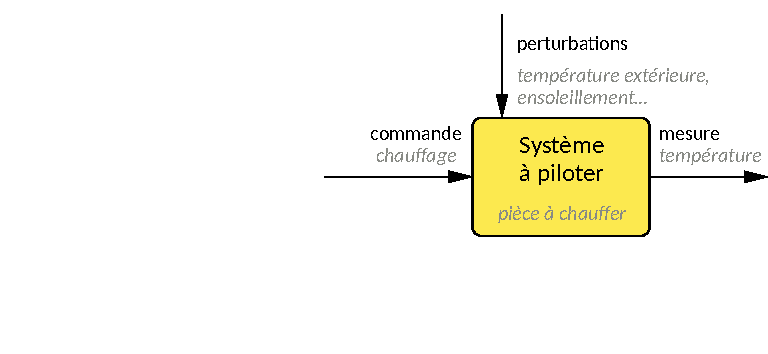
\includegraphics[width=\textwidth]{figures/MPC_sys.pdf}
    
    Au commencement: un système à piloter/commander
    }
  \only<2>{%
    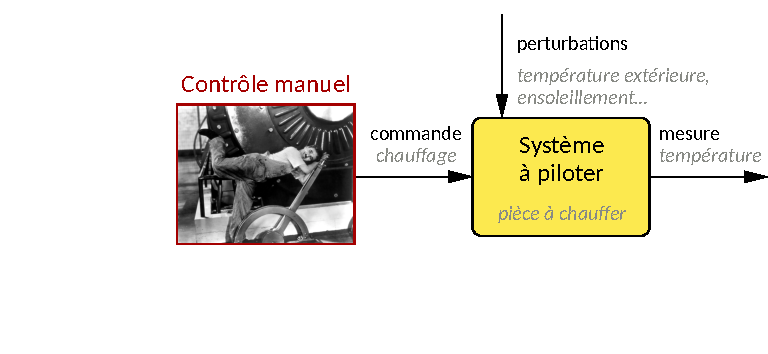
\includegraphics[width=\textwidth]{figures/MPC_man.pdf}
    
    On peut piloter le système à la main...\\
    
    }
  \only<3>{%
    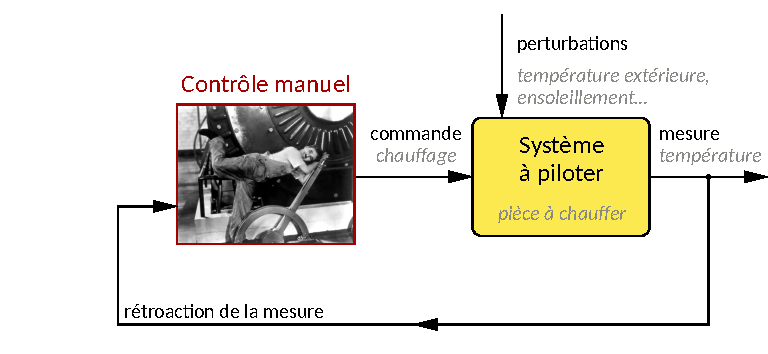
\includegraphics[width=\textwidth]{figures/MPC_fback.pdf}
    
    On peut piloter le système à la main...\\
    (on s'aide généralement de la mesure \\ → ``rétroaction'', ``boucle fermée'')
    }
  \only<4>{%
    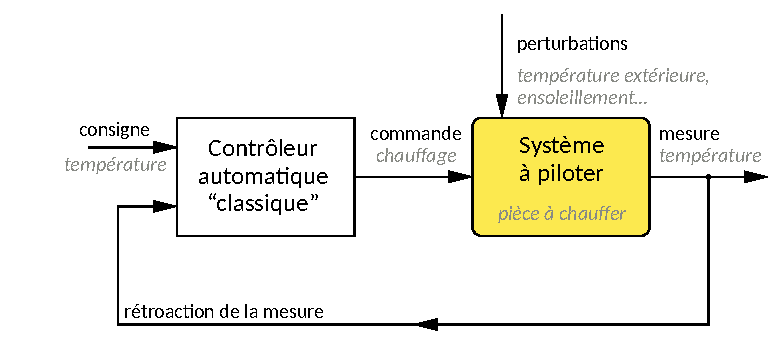
\includegraphics[width=\textwidth]{figures/MPC_classic.pdf}
    
    Commande automatique : génération de la commande\\
    pour suivre une \textbf{consigne}
    \detail{(PID: \textasciitilde 1930)}
    }
  \only<5->{%
    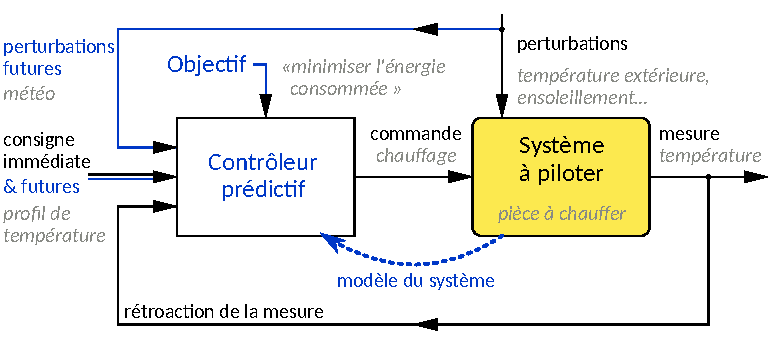
\includegraphics[width=\textwidth]{figures/MPC.pdf}
    
    Commande prédictive (\textasciitilde 1970) : le simple ``suivi de la consigne''\\ est remplacé
    par un \textbf{objectif à optimiser}\\ \detail{(à minimiser ou maximiser, selon l'objectif)}
    }
  \end{center}
\end{frame}

\begin{frame}
  \frametitle{Commande prédictive : les ingrédients}
  
  Le ``Model Predictive Control'' (MPC) se base sûr :
  \begin{itemize}
   \item \textbf{Objectif} (critère mathématique) à optimiser : \\
   coût économique, consommation, ...\\
   ou, plus classiquement, écart quadratique à une consigne,
   \item \textbf{Modèle de la dynamique} du système : influences des entrées commandées et extérieures (perturbations)
   \item \textbf{Prévisions} sur un horizon des consignes et perturbations futures
  \end{itemize}
  
  \bigskip \pause
  → Travail de conception plus élevé qu'avec une ``régulation classique''
 \emph{ (mais ça vaut le coup : très déployé industriellement)}.

\end{frame}

\begin{frame}
  \frametitle{Commande prédictive : besoin en calcul}
  
  Utilisation \emph{en ligne} d'un algorithme d'optimisation :
  
  \begin{block}{Optimisation ``en boucle fermée''}
  \begin{itemize}
   \item à chaque pas, calcul d’une \emph{séquence optimale} : \\
   commandes pour l’instant présent et les instants futurs
   \item seule la commande présente est effectivement appliquée
   \item au pas suivant, reprise du calcul sur l’horizon décalé \\(→ « horizon glissant »)
  \end{itemize}
  \end{block}
  
  \bigskip \pause
  → Nécessité d'embarquer de la \textbf{puissance de calcul}\\ \pause
  \detail{(mais on est en 2016)}
  
  \begin{center}
    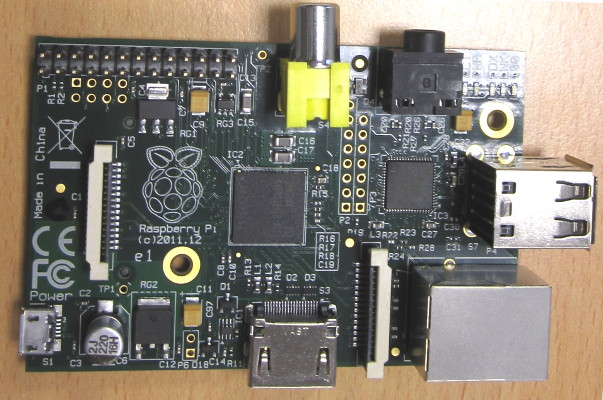
\includegraphics[width=0.25\textwidth]{figures/RPi_2013_02.jpg}
  \end{center}

\end{frame}

\begin{frame}
  \frametitle{Commande prédictive : mise en œuvre}
  
  Pour que l'optimisation \emph{en ligne} soit :
  \begin{itemize}
   \item fiable (pas de problème de convergence)
   \item soluble en un temps raisonnable (complexité polynomiale)
  \end{itemize}
  elle souvent formulée de façon \textbf{linéaire/quadratique}.
  
  \detail{(ça tombe bien : ``Coût = $\sum_k$ Prix$_k$ × \textbf{Puissance}$_k$ $\Delta_t$'' est linéaire)}
  
  \bigskip \pause
  → utilisation solvers de ``programmes linéaires/quadratiques'' :
  
  \begin{itemize}
   \item commerciaux : CPLEX (IBM), Gurobi
   \item libres : 
   \begin{itemize}
    \item GLPK (GNU) : programmes mixtes entiers linéaires ``MILP''
    \item ECOS (embotech) : dédié aux systèmes embarqués
    \item \textcolor{turquoise}{cvxopt : interface naturelle en Python} \\ { \footnotesize (Andersen, Dahl and Vandenberghe)}
   \end{itemize}
  \end{itemize}
\end{frame}

\begin{frame}
  \frametitle{Commande prédictive : en Python}
  
  NB : la R\&D en commande se fait souvent sous Matlab/Simulink :
  \begin{itemize}
   \item environnement puissant, riche en fonctionnalités \\(e.g. automatique et traitement du signal)
   \item mais commercial \detail{(et sémantique du language bof bof)}
  \end{itemize}

  \bigskip \pause
  
  Mais on peut s'en sortir en Python :
  
  \begin{itemize}
   \item calcul numérique avec des matrices : \textbf{numpy}
   \item solver d'optimisation linéaire : \textbf{cvxopt}\\
   (nb : interfaçage aux grands solvers commerciaux possible)
  \end{itemize}

\end{frame}


\section{Commande de chauffage en Python}

\begin{frame}
  \frametitle{Commande de chauffage classique}

\end{frame}

\begin{frame}
  \frametitle{Commande de chauffage prédictive}

\end{frame}


\section{Conclusion}



\begin{frame}[c]
  \frametitle{Conclusion}
  
  \begin{block}{La commande prédictive :}
  \begin{itemize}
   \item permet d'optimiser le pilotage d'un système\\ (e.g. économie de chauffage dans un bâtiment)
   \item peut se mettre en œuvre en Python \\(le gros du travail est dans un solver d'optimisation)
   \item peut se mettre en œuvre en Python avec des logiciels libres
  \end{itemize}
  \end{block}
  
  \pause
  \begin{block}{}
   → Vers de la domotique \emph{de commande} libre ?
  \end{block}


  
\end{frame}

\begin{frame}[c]
  \frametitle{Perspectives}
  
  Tester sur des Raspberry Pi\\ (→ travaux à Ulm Univ., mais code source non trouvé)
  
  \detail{
  (Hentzelt, Klingler, and Graichen,
  “Experimental Results for Distributed Model Predictive Control Applied to a Water Distribution System.”, 2014)}

  \bigskip
  
  Pour faciliter le travail :
  package \texttt{dmpc} \detail{(P. Haessig \& S.Chatel, 2016)}
  
  \begin{itemize}
   \item license BSD-3
   \item version alpha, mais déjà \texttt{pip install}-able depuis le dépot
   \item \url{https://github.com/pierre-haessig/python-dmpc}
  \end{itemize}
  
\end{frame}


\end{document}
